% \iffalse
\let\negmedspace\undefined
\let\negthickspace\undefined
\documentclass[journal,12pt,twocolumn]{IEEEtran}
\usepackage{cite}
\usepackage{amsmath,amssymb,amsfonts,amsthm}
\usepackage{algorithmic}
\usepackage{graphicx}
\usepackage{textcomp}
\usepackage{xcolor}
\usepackage{txfonts}
\usepackage{listings}
\usepackage{enumitem}
\usepackage{mathtools}
\usepackage{gensymb}
\usepackage{comment}
\usepackage[breaklinks=true]{hyperref}
\usepackage{tkz-euclide} 
\usepackage{listings}
\usepackage{gvv}                                        
\def\inputGnumericTable{}                                 
\usepackage[latin1]{inputenc}                               \usepackage{caption}
\usepackage{color}                                            
\usepackage{array}                                            
\usepackage{longtable}                                       
\usepackage{calc}                                             
\usepackage{multirow}                                         
\usepackage{hhline}                                           
\usepackage{ifthen}                                           
\usepackage{lscape}

\newtheorem{theorem}{Theorem}[section]
\newtheorem{problem}{Problem}
\newtheorem{proposition}{Proposition}[section]
\newtheorem{lemma}{Lemma}[section]
\newtheorem{corollary}[theorem]{Corollary}
\newtheorem{example}{Example}[section]
\newtheorem{definition}[problem]{Definition}
\newcommand{\BEQA}{\begin{eqnarray}}
\newcommand{\EEQA}{\end{eqnarray}}
\newcommand{\define}{\stackrel{\triangle}{=}}
\theoremstyle{remark}
\newtheorem{rem}{Remark}
\begin{document}

\bibliographystyle{IEEEtran}
\vspace{3cm}

\title{Audio Filtering}
\author{EE23BTECH11013 - Avyaaz$^{*}$% <-this % stops a space
}
\maketitle
\newpage
\bigskip

\renewcommand{\thefigure}{\arabic{figure}}
\renewcommand{\thetable}{\arabic{table}}

\bibliographystyle{IEEEtran}
\begin{table}[htbp]
% \setlength{\extrarowheight}{8pt}
\centering
 
\begin{tabular}{|c|c|}
\hline
\textbf{Parameter} & \textbf{Description}\\
\hline 
$x(n)$ & Input audio signal \\
\hline
$y(n)$ & Output audio signal\\
\hline
$H(e^{j\omega})$& Discret Time Fourier Transform of
$x(n)$\\
\hline
$h(n) $& Impulse response \\
\hline
\end{tabular}



 \caption{Parameters}
\label{tab:parameters}
\end{table}
\section{Spectrogram}
\begin{figure}[!h] 
\centering
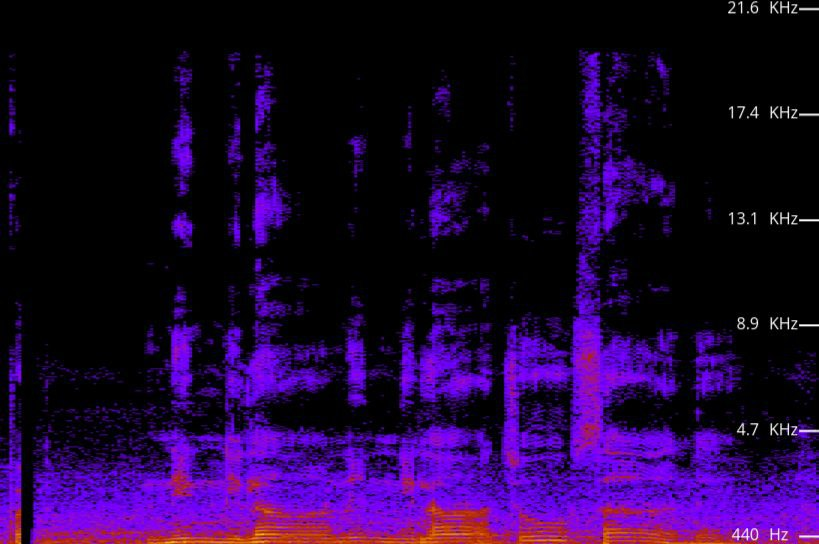
\includegraphics[width=\columnwidth]{figs/Input_audio_signal.jpg}
\caption{Spectrogram of input audio}
\end{figure}

\begin{figure}[!h] 
\centering
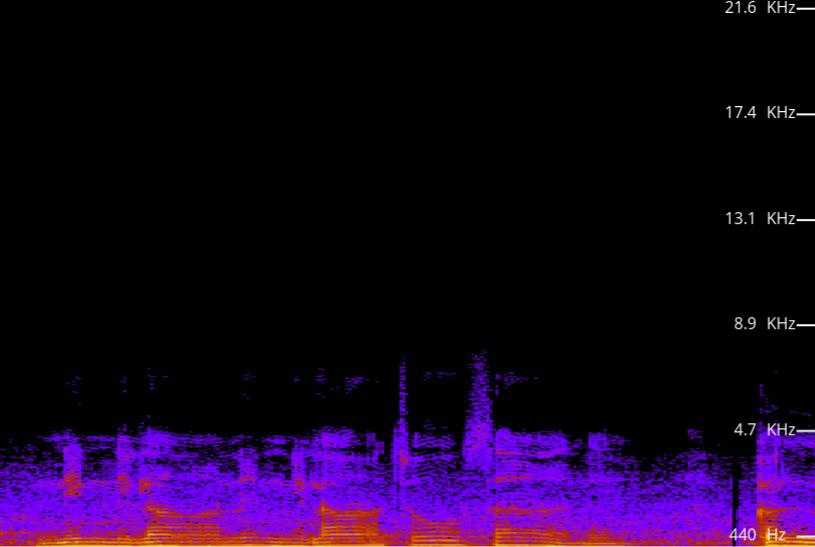
\includegraphics[width=\columnwidth]{figs/Output_audio_signal.jpg}
\caption{Spectrogram of output audio}
\end{figure}

The key strokes as well as
background noise is subdued in the audio.
% Also, the signal is blank for frequencies above
% 5.1 kHz.
\section{Digital Filter Input - Output}
$x(n)$ typically represents the input signal at
discrete time indices \(n\).

\begin{figure}[!h] 
\centering
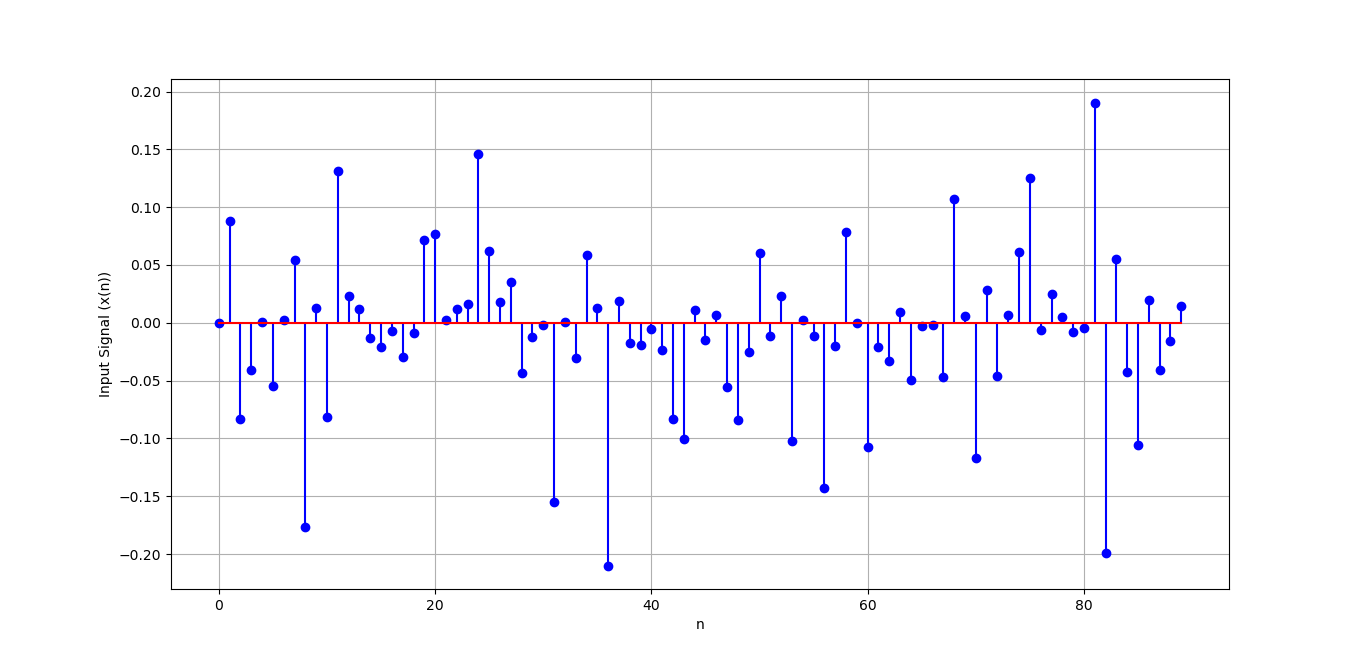
\includegraphics[width=\columnwidth]{figs/x(n).png}
\caption{Plot of $x(n)$  vs $n$ }
\end{figure}
Relationship between input and audio signal can be obtained from the difference equation: 
\begin{align}
     \sum _{m=0}^{M}a\brak{m}y\brak{n-m}=\sum _{k=0}^{N}b\brak{k}x\brak{n-k}
\end{align}
where, 
coefficients of $a$ and $b$ are obtained from the 'noise\_reduction.py'
\begin{align}
a &= [1, -2, 1, 0] \\
b &= [0.01, 0.05, 0.05, 0.01]
\end{align}
\begin{multline}
     y_{fwd}[n] = b[0]*x[n] + b[1]*x[n-1] + b[2]*x[n-2] \\+ b[3]*x[n-3] - a[1]*y_{fwd}[n-1] \\- a[2]*y_{fwd}[n-2] - a[3]*y_{fwd}[n-3]
\end{multline}
\begin{multline}
     y_{bwd}[n] = b[0]*y_{fwd}[n] + b[1]*y_{fwd}[n-1] + b[2]*y_{fwd}[n-2] \\+ b[3]*y_{fwd}[n-3] - a[1]*y_{bwd}[n+1]\\ - a[2]*y_{bwd}[n+2] -a[3]*y_{bwd}[n+3]
\end{multline}
\begin{align}
    y[n] = \frac{y_{fwd} + y_{bwd}}{2}\label{eq:iir_filter}
\end{align}

The forward and backward filtering operations are used in the implementation of the 'filtfilt' function to achieve zero-phase filtering.
% In the provided 'custom\_filtfilt' function, the forward filtering is applied first to the input signal x(n) using the given filter coefficients b and a. Then, the backward filtering is applied to the result obtained from the forward filtering.

\begin{figure}[htbp] 
\centering
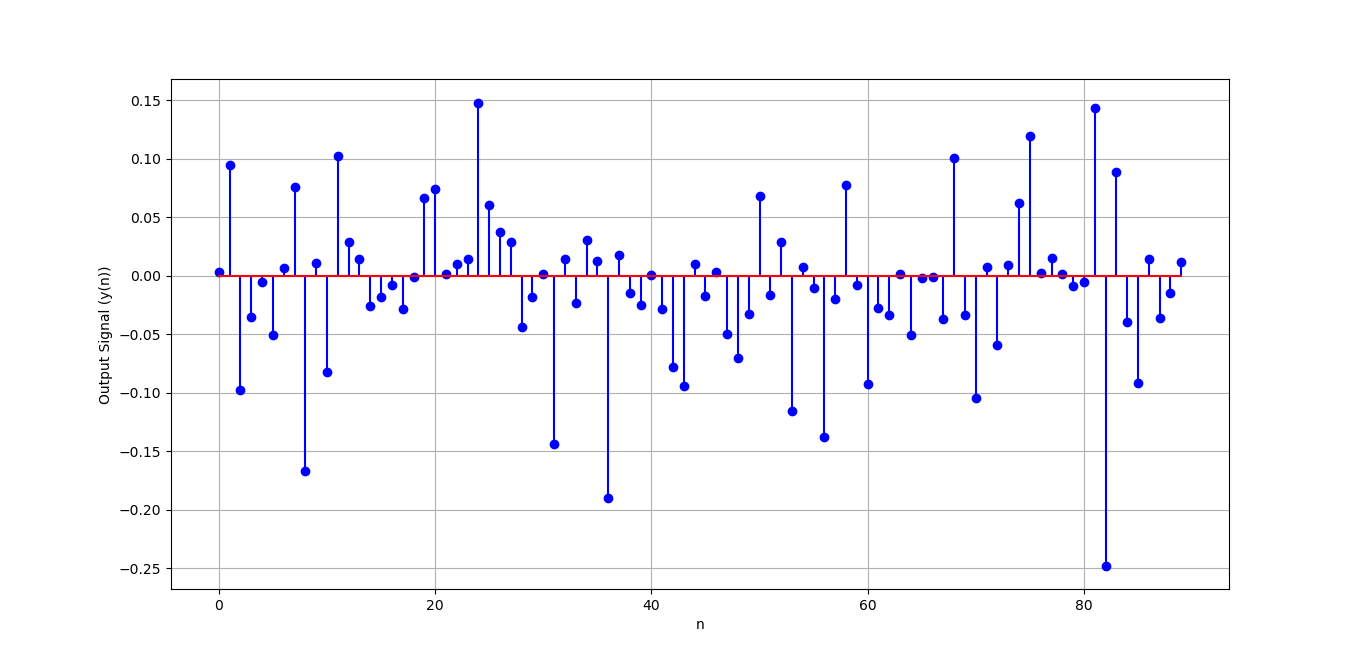
\includegraphics[width=1.1\columnwidth]{figs/y(n).png}
\caption{Plot of $y(n)$ vs $n$}
\end{figure}
% Here,
% \begin{align}
% x[n] & \system{\mathcal{Z}}(\omega) \\
% y[n] & \system{\mathcal{Z}}Y(\omega) \\
% h[n] & \system{\mathcal{Z}}\frac{Y(\omega)}{X(\omega)} = H(\omega)
% \end{align}
\section{Frequency Response}
\noindent We know that,
\begin{align}
\label{eq:z_trans_shift}
	{\mathcal {Z}}\{x(n-k)\} = z^{-k}X(z)
\end{align}
From  \eqref{eq:iir_filter}: Assuming that the $Z$-transform is a linear operation.
\begin{align}
    H(z) &= \frac{Y(z)}{X(z)}\\
    H(z) &= \frac{0.01z^{-3} + 0.05z^{-2}+0.05z^{-1}+0.01}{z^{-3}-2z^{-2}+z^{-1}} \quad ;|z|\neq 1,0\label{eq:H(z)}
\end{align}
Using,
\begin{align}
    H\brak{e^{j \omega}} = H\brak{z = e^{j \omega}}
\end{align}
\begin{figure}[htbp] 
\centering
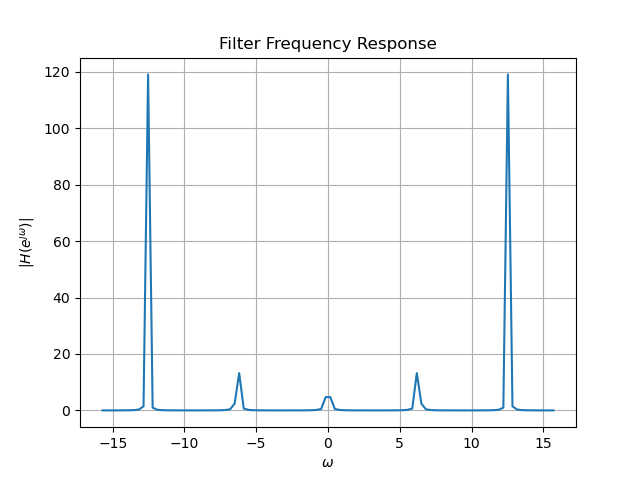
\includegraphics[width=\columnwidth]{figs/|H(z)|.png}
\caption{Plot of $|H(e^{j\omega})|$ vs $\omega$}
\end{figure}\\
\section{Impulse Response}
From equation \eqref{eq:H(z)}:
\begin{align}
    H(z) = 1 - \frac{1}{z^{-1}}
\end{align}

Taking inverse of $H(z)$:
\begin{align}
    H(z) \mathrel{\substack{\mathcal{Z}^{-1}\\\longleftrightarrow}} h(n)
\end{align}
\begin{align}
    h(n) = \delta(n) - \delta(n + 1)
\end{align}
\quad where,
\begin{align}
    \delta(n)
=
\begin{cases}
1 & n = 0
\\
0 & \text{otherwise}
\end{cases}
\end{align}
\begin{figure}[htbp] 
\centering
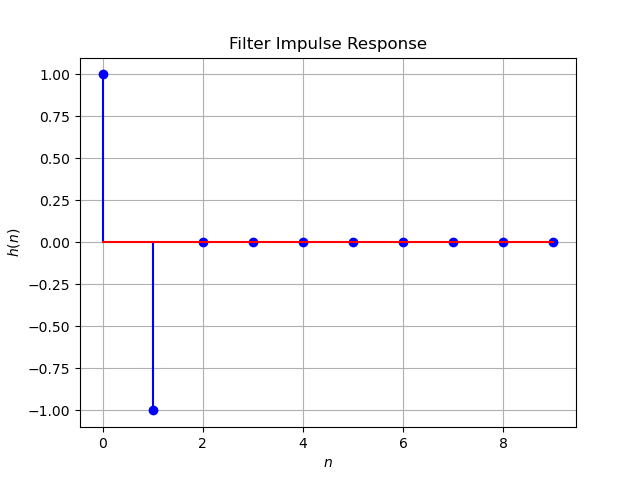
\includegraphics[width=\columnwidth]{figs/h(n).png}
\caption{Plot of $h(n)$ vs $n$}
\end{figure}

% \begin{multline}
%     h(n) = 0.01\delta(n) + 0.05\delta(n-1) + 0.05\delta(n-2) \\+ 0.01\delta(n-3) + 2h(n-1) - h(n-2)
% \end{multline}
\end{document}X
